%%
%% This is file `sample-vem.tex',
%% which is a modified version of `sample-sigconf.tex'.
%%
\documentclass[sigconf]{acmart} % The `anonymous' option is for double-blind review process.

\usepackage{multirow}
\usepackage[table,xcdraw]{xcolor}

\usepackage{mdframed}

\mdfsetup{skipabove=\topskip,skipbelow=\topskip}
\mdfdefinestyle{poistyle}{%
    frametitlerule=true,
}
\mdtheorem[style=poistyle]{poi}{Improvement}

%%
%% \BibTeX command to typeset BibTeX logo in the docs
\AtBeginDocument{%
  \providecommand\BibTeX{{%
    \normalfont B\kern-0.5em{\scshape i\kern-0.25em b}\kern-0.8em\TeX}}}


%% These commands are for a PROCEEDINGS abstract or paper.
% \acmConference[SBES'24]{Brazilian Symposium on Software Engineering}{September 30 -- October 04,  2024}{Curitiba, PR}

%%
%% end of the preamble, start of the body of the document source.


\settopmatter{printacmref=false} % This command was added for submissions to VEM
\setcopyright{none} % This command was added for submissions to VEM
\renewcommand\footnotetextcopyrightpermission[1]{} % This command was added for submissions to VEM



\begin{document}

%%
%% The "title" command has an optional parameter,
%% allowing the author to define a "short title" to be used in page headers.
\title{Can the Linux kernel sustain 30 more years of growth?
\\Toward mitigating bottlenecks in its development model}

\pagestyle{empty}


\begin{abstract}
    The Linux kernel, a Free Software project with over 30 years of active
    development, is central to modern computing. Together with system tools and
    utilities from the GNU Project, it forms the GNU/Linux ecosystem, which
    underpins critical social services, like the Internet, and is ubiquitous in
    cutting-edge computing fields. Linux development is driven by a global
    community of thousands of developers who collaborate primarily via email and
    mailing lists. This unique development model encompasses numerous processes
    and practices -  forming workflows - that go beyond the purely technical
    aspects of software development. Despite its success, the project depends
    heavily on critical workflows and key individuals, raising concerns about
    sustainability and workforce renewal. As the code base and community continue
    to grow in size and complexity, the entry barrier for newcomers and the
    workload for maintainers must not increase proportionally. Notably,
    significant time and effort are invested in developing tools to address
    limitations in the Linux kernel development model, challenges that are
    well-known to practitioners but remain underexplored in academic research.
    This paper presents our ongoing efforts to create taxonomies that accurately
    describe the workflows defining the Linux kernel development model. We also
    identify inherent bottlenecks and propose mitigation strategies by
    developing Free Software tools that support and sustain the Linux kernel
    ecosystem.
\end{abstract}

%%
%% Keywords. The author(s) should pick words that accurately describe
%% the work being presented. Separate the keywords with commas.
\keywords{Linux, Free Software, Linux kernel development model, Free Software
development model, software engineering, bottleneck mitigation.}

% \received{2 June 2024}
% \received[revised]{12 March 2009}
% \received[accepted]{5 June 2009}

%%
%% This command processes the author and affiliation and title
%% information and builds the first part of the formatted document.
\maketitle

\section{Introduction}

Computers are crucial devices that are pervasive in the modern world. Computer
systems range from personal computers that the general public uses for everyday
activities to embedded systems in a substantial portion of automobiles,
industrial devices, etc., performing critical tasks. While not a strict
requirement, computers commonly comprise two interacting parts: hardware and
software. The physical components of a computer constitute its hardware, while
the set of programs that control the operation of the hardware make up the
software. In this sense, software can adopt various forms to instruct hardware.

A piece of software common in most types of computers (including some embedded
systems) is an Operating System (OS). This typically vast and complex component
serves as a bridge between software applications and hardware. According to
\textit{Silberschatz (2008)}~\cite{silberschatz2008-operatingsystemconcepts},
``the operating system provides the means for proper use of these resources in
the operation of the computer system. An operating system is similar to a
government. Like a government, it performs no useful function by itself. It
simply provides an environment within which other programs can do useful work.''
The most important part of an OS is its kernel, which usually implements all
core functionalities and manages hardware support through device drivers.
\textit{Silberschatz (2008)}~\cite{silberschatz2008-operatingsystemconcepts}
also defines the kernel as ``the one program running at all times on the
computer.''

A prominent example of an OS kernel is the Linux kernel. As a Free Software
project, it can be fully modified and tailored, without licensing costs, for the
specific needs of individuals, companies, government agencies, and others. Linux
plays a central role in the operating system ecosystem and is backed by a large,
diverse group of stakeholders. It is foundational to critical services in modern
society, such as most of the Internet, and it dominates leading-edge fields like
Artificial Intelligence/Machine Learning (AI/ML), among others.

On the one hand, the Linux project continues to grow in size, complexity, and
number of contributors, which can be viewed as continuously evolving and
maturing. On the other hand, several concerns about its development model have
been raised by both academia and practitioners: (i) scalability of the community
and its workflows; (ii) workforce renewal; (iii) reliance on key individuals in
critical, often irreplaceable, roles; (iv) inefficiencies and wasted community
effort; (v) outdated technologies that remain core to the development process;
(vi) \textit{ad hoc} solutions to workflow bottlenecks and frequent duplication
of effort.

More severely, academic studies on the Linux project often lack engagement with
real-world practice and fail to investigate these concerns deeply, leading to
homogeneous and biased perspectives~\cite{wen2021-masterthesis}. Consequently,
academic conclusions sometimes diverge significantly from the experiences
reported in the Linux community (\textit{grey literature}) and insights from
close observation (\textit{ethnographic case
studies})~\cite{wen2021-masterthesis}. The widespread reliance on \textit{ad
hoc} solutions to common bottlenecks negatively impacts the scalability of both
workflows and the workforce, threatening the project's long-term sustainability.
In-depth academic research that bridges state-of-the-art and state-of-practice
could enable informed development of tools to support the Linux ecosystem and,
by extension, the many critical services of society that rely on Linux.

Given this gap in academic understanding, many topics remain underexplored or
superficially addressed in the literature. This work focuses on understanding
the overarching kernel workflows (i.e., the processes and practices required to
accomplish tasks) that define the Linux kernel development model. To that end,
we are building a theoretical framework to describe these workflows and identify
associated bottlenecks. Furthermore, we are designing and developing Free
Software tools to help mitigate these bottlenecks, leveraging insights grounded
in this framework.

While we recognize that achieving these objectives will not fully resolve all of
the aforementioned issues, our goal is to establish a concrete and empirically
grounded foundation upon which more comprehensive solutions can be built. Our
approach is multi-method, with a strong emphasis on \textit{ethnographic case
studies} to remain close to practice, while also integrating academic
literature, grey literature, and community insights to triangulate findings and
strengthen their validity.

This paper outlines our ongoing efforts to bridge the gap between research and
practice in the understanding of the Linux kernel development model. We aim to
inspire further investigation and collaboration on sustainable, community-driven
development of the tools that will help shape the next 30 years of Linux.

\section{Background}

The Linux kernel project is structured into interconnected subsystems analogous
to neighborhoods in a city~\cite{wen2021-masterthesis}, each managed by
maintainers responsible for overseeing developer contributions. These
maintainers and their associated code base areas are listed in the
\texttt{MAINTAINERS} file. However, entries in this file often overlap and share
code, forming clusters rather than isolated entities, which more accurately
represent subsystems~\cite{corbet2021-subsystems}. Reflecting its distributed
nature, the Linux community works in a decentralized, global, and asynchronous
fashion. Despite the natural coupling between parts of the code base, each
subsystem typically has a dedicated community and git repository (called
\textit{kernel tree}) with distinct governance, maintenance models, and
domain-specific characteristics.

\subsection{How the Linux kernel subsystems connect}

The Linux kernel project operates like a city divided into neighborhoods
(subsystems), each governed by maintainers and supported by their surrounding
ecosystems. Each subsystem operates as an autonomous project with its dedicated
kernel tree that synchronizes with the \textit{mainline} (the kernel tree of
Linus Torvalds, the creator of Linux) via pull requests\footnote{A request to
merge changes from one project fork into the original repository. Not to be
confused with \textit{GitHub Pull-Requests}.}. These subsystems manage specific
parts of the code base within a hierarchical \textit{web of trust}, where
responsibilities are delegated from higher to lower levels. Linus stands at the
top as a \textit{benevolent dictator}~\cite{corbet2014-4.4}, resolving disputes
and supervising the overall project direction. Despite this hierarchy, the
structure is flatter than it appears: many maintainers submit pull requests
directly to Linus, bypassing mid-level maintainers~\cite{corbet2017-patchflow}.
This recursive fragmentation of the top-level Linux project into smaller
projects gives it scalability and allows for highly specialized personnel caring
for every part of the code base. 

However, some inefficiencies have been detected, such as 44\% of contributions
being ignored over the past decade~\cite{rigby2014-peer-review}, which can
result in frustration and wasted community effort. This structure also makes the
whole project reliant on key, often irreplaceable individuals, particularly
Linus. 

In other words, even though this "divide-and-conquer" approach has contributed
to Linux's remarkable success, it exposes potential long-term risks, such as
maintainer overload and project fragility due to reliance on critical personnel.

\subsection{The Linux kernel development process}

At the core of the Linux kernel development process is the \textit{patch} - a
text document that describes the difference between two versions of the source
tree and represents a contribution to the project~\cite{wen2021-masterthesis}.
Like a git commit, a patch contains a code difference and a message, but it is
formatted for email submission.

In the Linux project, mailing lists are the medium for all public communication.
These mailing lists are hubs for development, bug reporting, and discussion.
Contributors submit patches for review, and maintainers and peers provide
feedback, initiating an iterative process known as the \textit{patch-reviewing
process}. This back-and-forth ensures high-quality
contributions~\cite{palix2011-faults-linux}, and once a patchset (a collection
of related patches) is accepted, it begins its path through the project's
hierarchical repository structure.

\begin{figure}[ht]
    \centering
    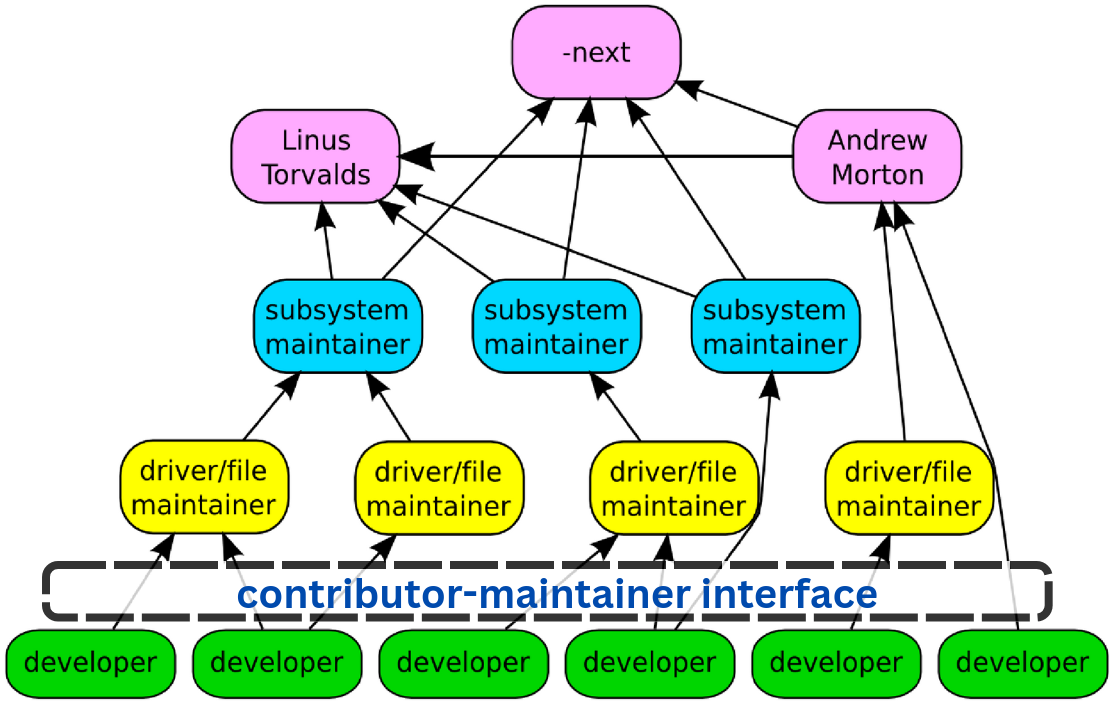
\includegraphics[width=0.45\textwidth]{images/patch-lifecycle.png}
    \caption{Patches flow into the \textit{mainline}~\cite{gregkh2016-patches-carved}.\label{fig:patch-lifecycle}}
\end{figure}

Initially, patches are merged into the corresponding subsystem repository under
the control of its maintainers. From there, they progress upward through the
hierarchy until they are merged into the \textit{mainline} repository.
\textbf{Figure~\ref{fig:patch-lifecycle}} illustrates this flow, highlighting
the patch journey from contributor to mainline. To prevent regressions and
ensure stability, \textit{Continuous Integration} (CI) practices, such as
temporary stabilization in the \texttt{-next} branches, are adopted.

Despite the rigor and success of this process, it is often considered outdated.
\textit{Izquierdo-Cortazar et al. (2017)}~\cite{izquierdo2017-review} advocate
for modernizing the review system, citing the limitations of mailing lists:
contributors must proactively subscribe to them, and issues related to email
delivery to subscribers are common. Solutions like the Lore kernel archives and
\textit{GitGitGadget} attempt to mitigate these problems by offering web-based
access to mailing lists and enabling contributions via \textit{GitHub
Pull-Requests}, respectively. These efforts underscore the growing demand for a
more accessible and efficient development workflows without compromising the
collaborative, decentralized nature of the project.

\subsection{The Linux kernel development model}

The Linux kernel development model encompasses a wide range of
\textit{workflows} that go beyond technical implementation. These include
submitting patches to mailing lists, following subsystem-specific guidelines,
and adhering to strict release cycles. While essential to maintaining structure
and quality, these workflows expose bottlenecks that limit efficiency. As noted
by \textit{Corbet and Kroah-Hartman
(2017)}~\cite{corbet-gregkh2017-linuxreport}, tooling is critical for managing
the complexity of a project as large and distributed as Linux, stating that
"Without the right tools, a project like the kernel would simply be unable to
function without collapsing under its own weight." Git is an example of a tool
devised in the Linux development context back in 2005, also created by Linus, to
replace the previous \textit{Version Control System} (VCS) used, and it has
since become a cornerstone of modern software development.

The community has developed and maintains various tools to cope with workflow
challenges. These range from official scripts, like \textit{get\_maintainers.pl}
(used to identify appropriate recipients for patches), to standalone projects,
such as \texttt{b4} (used for retrieving patches from archived mailing lists).
Developers also create \textit{ad-hoc} scripts to address specific personal
issues, often resulting in duplicated efforts and a lack of standardization. To
contribute to the scenario, we are actively developing Free Software tools such
as \textbf{Tool 1} and its subproject \textbf{Tool 2}, aiming to centralize and
streamline development workflows through a unified interface. These tools seek
not only to reduce inefficiencies but also to enhance the developer experience
sustainably and collaboratively.

\section{Research Design}

The Linux kernel project presents a unique organizational structure and a set of
collaborative development practices. However, as discussed in the previous
sections, it also reveals structural challenges and recurring bottlenecks that
may hinder its efficiency and long-term sustainability. These issues motivate
our research, which combines empirical methods with tool-supported interventions
grounded in the realities of kernel development. In this sense, we present the
two primary objectives of this work:

\begin{itemize}
    \item \textbf{Objective 1}: Validate a theoretical framework that accurately
    describes the overarching workflows of the Linux kernel development model
    and allows us to identify bottlenecks;
    \item \textbf{Objective 2}: Develop Free Software tools that efficiently
    mitigate bottlenecks in the Linux kernel development model using informed
    decisions based on a validated theoretical framework.
\end{itemize}

To guide the research work needed to accomplish these objectives, we designed
our study around the following two main research questions (RQs):

\paragraph{\textbf{RQ.1}: \textit{What overall workflows compose the Linux
kernel development model?}} This question aims to identify and characterize the
workflows that sustain the Linux kernel development process. These workflows
comprise technical and social processes and practices, from compiling and
installing a kernel from source code to patch submission and subsystem-specific
conventions. By answering RQ.1, we seek to build a comprehensive and structured
understanding of how development activities are coordinated across the
ecosystem.
    
\paragraph{\textbf{RQ.2}: \textit{Which processes and/or practices generate
bottlenecks in the Linux kernel development model that compromise its efficiency
and scalability?}} Building on the workflows mapped in RQ.1, this question
investigates the critical points where coordination, review, or tool limitations
slow development and reduce productivity. The aim is to uncover systemic
inefficiencies and understand how they impact maintainers, contributors, and the
overall project governance.

\paragraph{\textbf{RQ.2.1}: \textit{Which bottlenecks can be mitigated by
streamlining processes through automation?}} This subquestion explores
opportunities for improving the development experience by automating repetitive
and/or error-prone tasks. We examine whether automation can reduce delays, lower
entry barriers for contributors, or alleviate maintainer overload, thereby
increasing scalability and sustainability.



\subsection{Research methods}

This study adopts a multi-method qualitative approach combining two
complementary methods: (i) Ethnographic Case Studies (including participant and
non-participant observation) and (ii) a Multivocal Literature Review (MLR).

\subsubsection{Ethnographic case studies}

Ethnographic case studies provide an in-depth, context-sensitive understanding
of practices within a particular setting, combining methods such as observation,
interviews, and document analysis~\cite{edmonds2017-research-design}. In our
study, this approach draws on both direct involvement in the Linux ecosystem
(\textit{participant observation}) and interactions with contributors and
documentation analysis without direct engagement (\textit{non-participant
observation}).

For instance, we are conducting participant observation, interacting and
contributing (sending patches) with AMD GPU and IIO (Industrial I/O) subsystems.
The goal is to document experiences, interactions, and challenges in a
contribution journal. In parallel, we maintain two ongoing side projects,
\textbf{Tool 1} and \textbf{Tool 2}, as additional sources of insights into
kernel workflows and tool-supported processes and practices.

We are also investing in non-participant observation comprised of three
complementary strategies:

\begin{enumerate}
    \item \textbf{Mentoring newcomers}: Support and observe new contributors,
    cataloging experiences from the mentors' and mentorees' perspectives;
    \item \textbf{Empirical trials}: Conduct experiments with newcomers and
    experienced developers to evaluate how the proposed tools support workflows
    and mitigate bottlenecks. Newcomer feedback will be gathered through
    questionnaires; data from veteran developers will be collected via
    interviews and anonymized telemetry, following the model of the
    \textit{Debian Popularity
    Contest}\footnote{\href{https://popcon.debian.org/}{Debian Popularity
    Contest website}.};
    \item \textbf{Community engagement}: Participate in key community events to
    interact with core developers and gather qualitative feedback, as the Linux
    Foundation Technical Advisory Board (TAB) recommended to our research group
    regarding how we should approach collecting feedback from the Linux
    community.
\end{enumerate}

\subsubsection{Multivocal Literature Review (MLR)}

The MLR complements the ethnographic case studies methods by synthesizing
evidence from academic literature and Grey Literature (e.g., blogs, mailing
lists, conference talks). It combines the rigor of Systematic Literature Review
(SLR) with the breadth of Grey Literature Review (GLR)~\cite{vahid2018-mlr}.
Building on Wen's earlier MLR~\cite{wen2021-masterthesis}, we are conducting an
updated review focused on development workflows in the Linux kernel. This review
supports triangulation, allowing us to compare empirical findings with academic
and practitioner perspectives to reduce bias and strengthen the study's
validity.

\section{Phases and Current Progress}
\label{chp:workplan-schedule}

This work combines two research methods and the concurrent development of Free
Software tools. \textbf{Figure~\ref{fig:research-work-plan}} summarizes the four
planned phases of our research. Each phase comprises activities (such as
workflow mapping or tool development) centered around a core theme. All phases
culminate in an iteration of our theoretical framework for the Linux workflows
while leveraging these refined iterations to make informed decisions on the
development of the aforementioned tools. At the time of writing, Phase~1 has
been completed, while Phases~2 and~3 are ongoing.

\begin{figure}[ht]
    \centering
    \includegraphics[width=0.5\textwidth]{images/phd-phases.pdf}
    \caption{Description of the research work in phases.\label{fig:research-work-plan}}
\end{figure}

\subsection{Phase I: Exploratory immersion}
\label{sec:workplan-schedule:phase1}
This phase focused on engaging with the Linux kernel ecosystem, mentoring
newcomers, and developing \textbf{Tool 1} and \textbf{Tool 2}.

\paragraph{P1.1: Exploration of the Linux ecosystem}
We engaged with the ecosystem by submitting exploratory patches to subsystems
like AMD GPU, IIO, and staging. We also studied the experiences of other
contributors through blogs, papers, and direct conversations.

\paragraph{P1.2: Mentoring newcomers I}
In early 2024, during our \textit{Free Software Development} course, we mentored
about 30 students through setting up a development environment, developing a
patchset, sending it as a contribution, and participating in the review process
of Linux. This approach included in-person workshops with veteran developers.
Students completed an anonymous survey and wrote blog posts to report their
experiences.

\paragraph{P1.3: Tools development I}
We actively developed \textbf{Tool 1} and mentored two contributors through
\textit{Google Summer of Code} (GSoC). \textbf{Tool 2} was extracted from
\textbf{Tool 1}, rewritten in Rust, and evolved into a standalone project with
improved performance and stronger community engagement.

\subsection{Phase II: Deeper immersion}
In this phase, we aim for deeper technical involvement and to introduce
controlled experiments with newcomers.

\paragraph{P2.1: Deeper contributions and maintainer role}
We are submitting more impactful patches and participating in code reviews to
simulate maintainer responsibilities. Our goal is to naturally escalate our
involvement in the ecosystem.

\paragraph{P2.2: Mentoring newcomers II}
A second iteration of the mentoring course is being offered in 2025,
incorporating lessons learned from the first edition.

\paragraph{P2.3: Experiments I (newcomers)}
During the second iteration of the mentoring course, half the students were
randomly assigned to use \textbf{Tool 1}, while the rest used the original
(unassisted) toolset. A survey is being used to collect data to validate the
hypothesized workflow bottlenecks and measure if and how \textbf{Tool 1}
mitigated them, both qualitatively and quantitatively.

\paragraph{P2.4: Tools development II}
With clearer insights into workflows, \textbf{Tool 1} is being stabilized, and
\textbf{Tool 2} is being expanded. We are mentoring another contributor through
GSoC 2025, focusing on \textbf{Tool 2} improvements.

\subsection{Phase III: Unbiasing through external validation}
This phase cross-validates findings from previous phases with external sources
to reduce bias.

\paragraph{P3.1: Multivocal Literature Review}
We are conducting an updated MLR focused on kernel development workflows,
combining academic publications and grey literature such as blogs and mailing
lists.

\paragraph{P3.2: Community feedback at events}
Following the recommendation from the Linux Foundation's TAB, we are
participating in events such as
\textit{FOSDEM 2025}\footnote{\href{https://fosdem.org/2025/}{FOSDEM 2025}} and
\textit{DebConf 2025}\footnote{\href{https://debconf25.debconf.org/}{DebConf
2025}}, ideally as speakers presenting \textbf{Tool 1} and \textbf{Tool 2} to
collect direct feedback from experienced kernel developers and key personnel of
the community.

\paragraph{P3.3: Tools development III}
We will refine the tools based on insights from the first iteration of our
taxonomy and community feedback.

\subsection{Phase IV: Final validation in real-world scenarios}
The final phase aims to validate the improved taxonomy through experiments with
experienced kernel developers.

\paragraph{P4.1: Experiments II (veteran developers)}
Veteran developers will use \textbf{Tool 1} and \textbf{Tool 2} in their regular
workflows. Usage data will be collected via \textbf{Tool 1}'s data collection
(e.g., compilation frequency and duration) and local storage infrastructure.
This collected data will be sent to servers using its telemetry features and
analyzed. A data anonymization mechanism inspired by the \textit{Debian
Popularity Contest} is being designed.

\paragraph{P4.2: Tools development IV}
Based on the refined taxonomy from earlier phases, we will finalize tool
development to align with real-world kernel development practices.

\section{Preliminary Results and Discussion}

In this section, we present and discuss the early results of our research work.

\subsection{Empirical evidence of long-term unsustainability}

We have produced empirical quantitative evidence indicating that the Linux
kernel development model may be unsustainable due to its current
structure\footnote{These experiments are reproducible with \textit{Docker}
following the instructions in the anonymized git repository pointed in the
\textit{Artifacts Availability} section.}. \textbf{Figures \ref{fig:loc-linux}},
\textbf{\ref{fig:maintainers-linux}}, and \textbf{\ref{fig:commits-linux}} are
plots that show statistics about the development of Linux over the last 10
years. Due to the periodicity of releases that follow subsequent six to
eight-week cycles, we can use the Linux versions as consistent timestamps to
analyze the evolution of the project. In this sense, the aforementioned figures
have the Linux versions in the abscissa from 3.19 (launched on 8 February 2015)
until 6.13 (launched on 20 January 2025).

\begin{figure}[ht]
    \centering
    \includegraphics[width=0.45\textwidth]{images/phys-loc.pdf}
    \caption{Linux logical Lines of Code (LLOC) from version 3.19 to 6.13.\label{fig:loc-linux}}
\end{figure}

\textbf{Figure \ref{fig:loc-linux}} displays the increase of \textit{logical
Lines of Code} (LLOC)\footnote{A software metric that measures the number of
source lines of code (excluding blank ones and comments) in a program source
code.} and shows how the Linux kernel code base is steadily growing regarding
its size. We can derive that the project complexity is also growing as more
features, drivers, and the like are continuously being merged.  Interestingly,
by investigating the entries in the \texttt{MAINTAINERS} file, we produced
\textbf{Figure \ref{fig:maintainers-linux}} that depicts how the number of
maintainers steadily increases.

\begin{figure}[ht]
    \centering
    \includegraphics[width=0.45\textwidth]{images/maintainers.pdf}
    \caption{Number of Linux maintainers from version 3.19 to 6.13.\label{fig:maintainers-linux}}
\end{figure}

Notwithstanding the increase in the number of maintainers, we can see in
\textbf{Figure \ref{fig:commits-linux}} that the amount of commits in each
development cycle of Linux fluctuates between 13000 and 17500 since version
3.19, excluding outliers.  Every commit is different as an individual commit can
be a massive change, while a set of ten commits can be a single line change ten
times, and a difference of four and a half thousand commits is expressive, so we
can not derive solid conclusions based on these statistics. However, just the
fact that the number of commits has fluctuated consistently indicates that the
contribution throughput does not scale in the same fashion as the number of
maintainers. We can hypothesize that, as time passes, parts of the code base do
not receive maintenance for long periods, either because they are abandoned or
have reached great stability; no matter the case, this would still incur in the
growing proportion of maintainers per LLOC (in this scenario, LLOC would, at
least, not grow accordingly) not translating in more code productivity.

\begin{figure}[ht]
    \centering
    \includegraphics[width=0.45\textwidth]{images/commits.pdf}
    \caption{Commits in the development cycle of versions 3.19 to 6.13.\label{fig:commits-linux}}
\end{figure}

The Linux kernel development model functions as a self-sustaining and highly
specialized ecosystem. However, by extrapolating the empirical evidence, we can
assume that the model reliance on a continuous influx of skilled contributors, a
highly dedicated pool of maintainers, and ever-increasing code complexity
suggests characteristics similar to an ``economic bubble'' where short-term
growth may mask long-term sustainability risks.

\subsection{Core overall workflows}

\begin{figure}[ht]
    \centering
    \fbox{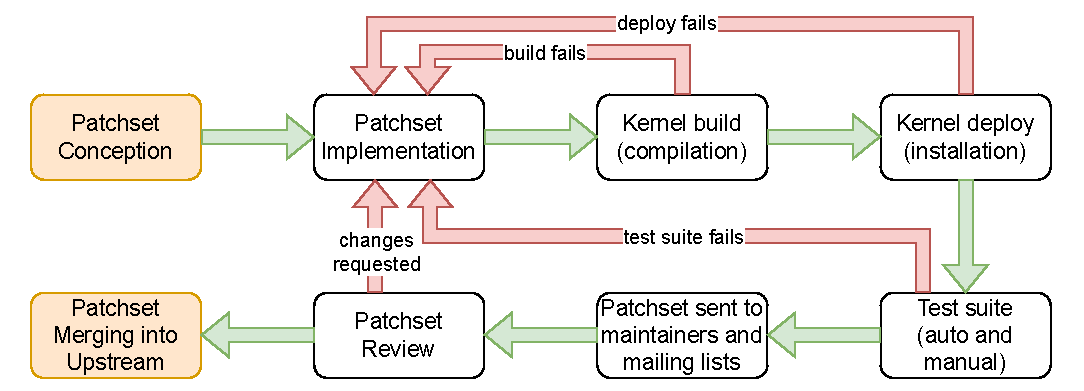
\includegraphics[width=0.8\linewidth, 
    clip=true, trim= 0px 5px 0px 5px]
    {images/patchset-development-workflow.pdf}}
    \caption{Concept map of the patchset development workflow.}
    \label{fig:patchset-dev-workflow}
\end{figure}

We have extensive experience with the Linux ecosystem from both industry and
academic perspectives. By actively contributing to and even assuming maintainer
responsibilities in subsystems such as \textit{AMD GPU}, \textit{Industrial I/O
(IIO)}, and \textit{Virtual Kernel Mode Setting} (VKMS), along with conducting
research in Free Software, in special, Linux, many insights emerge. 

\begin{figure}[ht]
    \centering
    \fbox{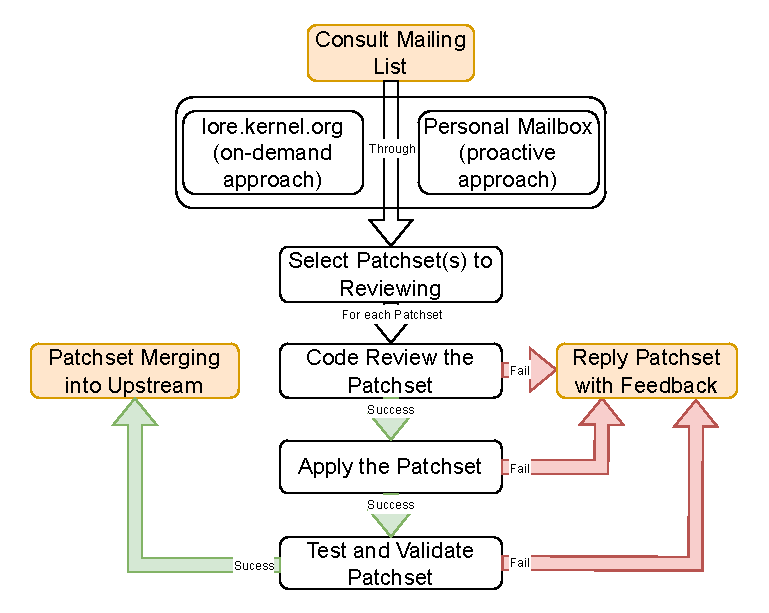
\includegraphics[width=0.8\linewidth, 
    clip=true, trim= 0px 5px 0px 5px]
    {images/patchset-reviewing-workflow.pdf}}
    \caption{Concept map of the patchset reviewing workflow.}
    \label{fig:patchset-rev-workflow}
\end{figure}

Building from those, the work done in Phase~1 (as described in
\textbf{Section~\ref{sec:workplan-schedule:phase1}}) formalized the two core
overall workflows, which are the \textit{patchset development workflow}
(\textbf{Figure~\ref{fig:patchset-dev-workflow}}) and the \textit{patchset
reviewing workflow} (\textbf{Figure~\ref{fig:patchset-rev-workflow}}) as concept
maps. The former relates to contributors' work, while the latter relates to
maintainers' work.

Due to the vastness and diversity of the Linux subsystems, these workflows can
mutate depending on the context-specific needs and characteristics; as such, we
denominate them as \textit{overall}.

\subsection{Development of supporting tools}

Drawing from the same sources as the previous section, we developed
\textbf{Tool 1}, a \textit{Developer Automation Workflow System} (DAWS)
designed to streamline and automate workflows for Linux developers. It provides
a unified interface offering solutions to common kernel development challenges,
such as abstracting hardware and distribution-specific complexities for tasks
like configuring, compiling, and installing custom kernels. It also includes
tools for submitting contributions and managing reviews, which have gained
traction among industry developers. We also developed \textbf{Tool 2}, a
\textit{Terminal User Interface} (TUI), designed for maintainers, that
simplifies the interaction with patches sent to mailing lists and review
management, addressing one of the most critical bottlenecks in the development
model.

From the users' perspective, \textbf{Tool 1} is built as a hub-like tool that
provides a set of commands covering many aspects of the kernel workflows. For
instance, there are commands to streamline and automate the tasks of compiling
and installing a kernel from the source code, as well as commands to manage
configuration files, target machines, and much more. Even though we singled out
\textbf{Tool 2} throughout the text, it still is a command of \textbf{Tool 1},
only with the distinctive characteristic of being a dedicated sub-project with a
different software stack and more abrangent scope, compared with the other
commands.

From the developers' perspective, \textbf{Tool 1} can still be viewed as a hub
due to its modularized and extensible architecture incorporating robust existing
tools that already solve Linux developers' pain points. In this regard, the
project suppresses duplication of efforts while providing high-quality solutions
to users and enhancing maintenance for its developers.

\textbf{Tool 1} also has a comprehensible and extensible infrastructure to
(locally) collect data points that could be of interest for research into the
workflows of the Linux kernel development model. For example, the time of
compilation and whether it was successful is currently collected by \textbf{Tool
1} and can be used to derive results about the compilation of the kernel task.
Another interesting data point regarding compilation could be hardware setups
and cross-compilation tracking, allowing for deep analysis of the efficiency of
hardware setups and compiler use.

\section{Conclusion}
\label{sec:conclusion}

This paper outlines an ongoing research effort to understand and support the
sustainability of the Linux kernel - a project central to many fields in
Computer Science and the society at large. Recognizing the complexity and scale
of this Free Software ecosystem, we have proposed a research work plan grounded
in empirical and non-empirical methods, with the goals of developing and
validating a theoretical framework for the workflows that govern the Linux
kernel development model (Objective 1) and designing tools that mitigate
identified bottlenecks (Objective 2). While our findings are preliminary, they
have revealed signs of concern about the project's continued growth and its
long-term sustainability. These insights - derived from participant and
non-participant observations - motivate deeper investigation into how workflows
function in practice, how they differ across subsystems, and where they inhibit
scalability by generating bottlenecks.  The theoretical framework under
construction serves not only as a lens through which to describe and analyze the
Linux development model but also as a foundation for informed decisions in
developing supporting tools. We see this framework as a contribution of enormous
potential, capable of bridging the gap between state-of-the-art and
state-of-the-practice, which is often fragmented in the context of Free Software
development. By sharing this work-in-progress, we invite feedback from the
Software Engineering community and aim to spark discussion on the challenges of
sustaining large, community-driven Free Software projects. Insights from the
Linux kernel can guide robust tool development and further scientific research.
We aim to contribute to this effort by combining empirical observation,
theoretical grounding, and tooling experimentation.

\section*{Artifacts Availability}

To reproduce the experiments that generated the Linux project statistics, visit
the anonymized repository pointed by this URL:
\url{https://anonymous.4open.science/r/linux-stats-0678/}. After accessing the
anonymized repository, locally download it with the \textit{Download Repository}
button, then follow the instructions described in the file
\texttt{linux-stats/README.md}. The only requirements to run these experiments
are \texttt{docker} and \texttt{docker-compose}.

%\begin{acks}
%The authors of this paper have received financial support from FAPESP under the %research grant 2024/00957-8.
%\end{acks}

%%
%% The next two lines define the bibliography style to be used, and
%% the bibliography file.
\bibliographystyle{ACM-Reference-Format}
\bibliography{references}

\end{document}
\endinput
